\documentclass[12pt,a4paper]{ctexart}
%宏包
\usepackage{amsmath}%数学符号
\usepackage{amssymb}%数学符号
\usepackage{amsthm}%数学符号
\usepackage{geometry}%界面布局
\usepackage{natbib}%bibtex
\usepackage{tikz}%交换图
\usepackage{tikz-cd}%交换图
\usepackage{quiver}%交换图
\usepackage{float}%浮动体固定
\usepackage{caption}%图片标题
\usepackage[colorlinks,linkcolor=blue]{hyperref}%超链接
\usepackage{enumerate}%计数列表
\usepackage{tabularx}%控制列宽
\usepackage{xr}%跨文件引用
% \externaldocument{D:/latex/book/algebra/algebra}
% \externaldocument{D:/latex/book/analysis/analysis}
% \usepackage{CTEX}
% \ctexset{today=old,contentsname=Contents}
   
%页面设置
\linespread{1.2}
\geometry{a4paper,left=2cm,right=2cm,top=2.5cm,bottom=2cm}
%\geometry{a4paper,left=2cm,right=2cm,top=2.5cm,bottom=2cm}

%环境和宏指令
\newenvironment{prooff}{{\noindent\it\textcolor{cyan!40!black}{Proof}:}\,}{\par \vskip 1cm}
\newenvironment{proofff}{{\noindent\it\textcolor{cyan!40!black}{Proof of the lemma}:}\,}{\qed \par}
\newcommand{\bbrace}[1]{\left\{ #1 \right\} }
\newcommand{\bb}[1]{\mathbb{#1}}
\newcommand{\p}{^{\prime}}
\renewcommand{\mod}[1]{(\text{mod}\,#1)}
\newcommand{\blue}[1]{\textcolor{blue}{#1}}
\newcommand{\spec}[1]{\text{Spec}({#1})}
\newcommand{\rarr}[1]{\xrightarrow{#1}}
\newcommand{\larr}[1]{\xleftarrow{#1}}
\newcommand{\emptyy}{\underline{\quad}}
\newenvironment{enu}{\begin{enumerate}[(1)]}{\end{enumerate}}
%ctrl+点击文本返回代码  选中代码 ctrl+alt+j 为代码查找文本

%定理环境
\theoremstyle{definition}
\newtheorem{defn}{Definition}[section]
\newtheorem{coro}[defn]{Corollary}
\newtheorem{theo}[defn]{Theorem}
\newtheorem{exer}[defn]{Exercise}
\newtheorem{rema}[defn]{Remark}
\newtheorem{lem}[defn]{Lemma}
\newtheorem{prop}[defn]{Proposition}
\newtheorem{nota}[defn]{Notation}
\newtheorem{exam}[defn]{Example}

\begin{document}

\title{Hecke L函数的解析延拓}
\author{}
\date{}
% \thispagestyle{empty}
% \begin{figure}
%     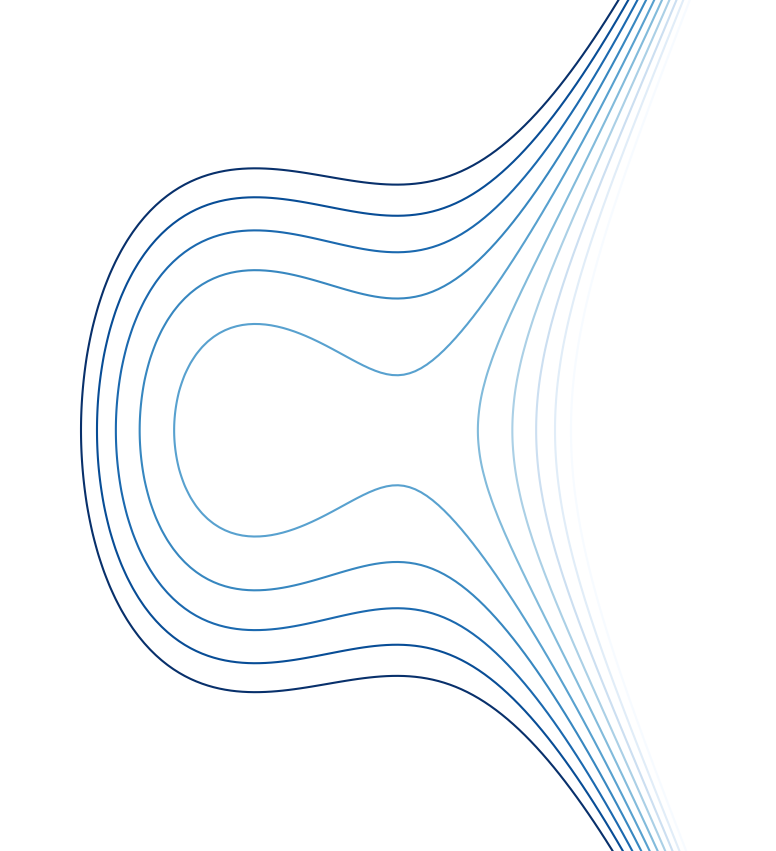
\includegraphics{cover.png}
%     \centering
% \end{figure}
\maketitle
\section{课题的背景、意义及培养目标}
John Tate在他1950年的博士论文中, 综合运用了代数数论, 拓扑群上调和分析的方法给出
Hecke $L$函数解析延拓的全新证明, 
是现代自守形式的开篇之作。 
本课题主要研究Tate这篇博士论文的动机背景以及技术细节。
\section{设计(论文)的原始数据与资料}
主要参考文献为Tate的原始论文以及一些辅助材料,比如Weil的Basic Number Theory, 以及MIT教授Poonen
的笔记。 
其中原始论文可以在Cassels的Algebraic Number Theory最后一章找到。

\cite{MR1397028}\cite{MR1680912}\cite{MR217026}\cite{MR427267}

\section{课题的基本要求}
\begin{enu} 
    \item 系统阅读 Tate's thesis, 理解论文的整体结构和核心思想。
    \item 梳理和总结其中关键理论, 
    如Adele和Idele的定义与性质,Hecke L 函数的解析延拓与函数方程, 
    以及Dedekind zeta函数$\zeta_K(s)$在$1$处留数表达式的证明。
    \item 提出并解答阅读过程中遇到的理论问题。
    \item 撰写数学读书笔记。
\end{enu}

\section{完成任务后提交的书面材料要求}
\begin{enu} 
    \item 展现对 Tate's thesis 的深入理解,能清晰阐述论文的核心内容。
    \item 数学表达规范,推导与证明完整无误,书写格式符合毕业设计规范。
    \item 突出个人的数学思考能力,适当补充与拓展相关问题的内容。
    \item 文献综述与引用符合学术规范。
\end{enu}




\bibliography{renwu}
\bibliographystyle{plain}%终端输入bibtex+文件名再ctrl+s两次



\end{document}